\documentclass[ngerman,twocolumn,showpacs,%
  nofootinbib,aps,superscriptaddress,%
  eqsecnum,prd,notitlepage,showkeys,10pt,report]{revtex4-2}


\usepackage{amssymb}
\usepackage{amsmath}
\usepackage{graphicx}
\usepackage{dcolumn}
\usepackage[hidelinks]{hyperref}
\usepackage{listings}
\usepackage{color}
\usepackage{csvsimple}
\usepackage{booktabs}
\usepackage{longtable}
\usepackage{fancyvrb}
\usepackage{makeidx}
\usepackage[ngerman]{babel}
\usepackage{tocbasic}
\usepackage[export]{adjustbox}

\definecolor{dkgreen}{rgb}{0,0.6,0}
\definecolor{gray}{rgb}{0.5,0.5,0.5}
\definecolor{mauve}{rgb}{0.58,0,0.82}

\DeclareTOCStyleEntries[
  %raggedentrytext,
  numwidth=0pt,
  numsep=1ex,
  dynnumwidth
]{tocline}{chapter,figure,table}

\DeclareTOCStyleEntries[
  %raggedentrytext,
  numwidth=0pt,
  numsep=1ex,
  dynnumwidth,
  indent=0pt,
  dynindent,
]{tocline}{section,subsection,subsubsection,paragraph,subparagraph}

\lstset{frame=tb,
  language=Python,
  aboveskip=3mm,
  belowskip=3mm,
  showstringspaces=false,
  columns=flexible,
  basicstyle={\scriptsize\ttfamily},
  numbers=none,
  numberstyle=\tiny\color{gray},
  keywordstyle=\color{blue},
  commentstyle=\color{dkgreen},
  stringstyle=\color{mauve},
  breaklines=true,
  breakatwhitespace=true,
  tabsize=3
}
\lstset{literate=%
    {Ö}{{\"O}}1
    {Ä}{{\"A}}1
    {Ü}{{\"U}}1
    {ß}{{\ss}}1
    {ü}{{\"u}}1
    {ä}{{\"a}}1
    {ö}{{\"o}}1
    {~}{{\textasciitilde}}1
}

\begin{document}
\renewcommand*{\tocname}{Inhaltsverzeichnis}
\renewcommand*{\lofname}{Abbildungsverzeichnis}

\title{Citizen Science, Open Data und Geschlechtergerechtigkeit - \\
Straßennamen in Aschaffenburg: Eine Analyse der Namensgebung\\
mit Hilfe von OpenStreetMap und Wikidata}
\author{Fabi Hahner}


\begin{abstract}
Das Ziel in der vorliegenden Arbeit ist es, zu klären, ob es bei der Namensgebung von
Straßen, Plätzen, Schulen und anderen geographisch kartierbaren Orten im Stadtbereich
Aschaffenburg Auffälligkeiten gibt und ob dabei Fragestellungen wie
Geschlechtergerechtigkeit und Parteizugehörigkeiten berücksichtigt werden.
Um die Forschungsfragen zu beantworten, wurden die Straßennamen in einer Studie auf
ihre Etymologie untersucht und mit öffentlich zugänglichen Datenbanken abgeglichen.
Die Studie zeigte, dass im untersuchten Gebiet überdurchschnittlich viele Straßen nach
Cis-Männern und NSDAP-Mitgliedern benannt wurden. Dies zeigt, dass die
Entscheidungsträger*innen in der Vergangenheit bei der Auswahl von Straßennamen
voreingenommen waren.\\
Auf dieser Grundlage ist es empfehlenswert, zukünftige Straßenbenennungen bzw.
-umbenennungen so zu planen, dass nicht-männliche Namensgeber*innen
überdurchschnittlich stark berücksichtigt werden, um langfristig einen gerechten Ausgleich
zu erreichen. Zudem ist es empfehlenswert, Straßen und andere Orte, die nach
NSDAP-Mitgliedern benannt wurden, umzubenennen, da deren Beibehaltung dem Ansehen
der Stadt schaden könnte.
\end{abstract}

\maketitle


\tableofcontents
\listoffigures
\newpage

\section{Datenerhebung}

Die der Untersuchung zugrundeliegenden Werkzeuge sind OpenStreetMap\footnote{\url{https://www.openstreetmap.org/}} (nachfolgend
“OSM” genannt) und Wikidata\footnote{\url{https://www.wikidata.org}}. Als Quelle dient die Website des Stadtarchivs\footnote{\url{https://aschaffenburgzweinull.stadtarchiv-digital.de/projekt/strassennamen-in-aschaffenburg/}}.
OSM ist eine öffentlich zugängliche Geodatenbank, in der Metadaten zu allen geographisch
kartierbaren Dingen gespeichert werden können. Daraus lassen sich nicht nur Karten
erstellen, sondern viele andere geographisch bestimmbare Analysen durchführen.
Wikidata ist eine öffentlich zugängliche Wissensdatenbank, die eng mit der Wikipedia
verknüpft ist und - beispielsweise - biographische Daten zu historischen und Personen des
öffentlichen Lebens in maschinenlesbarer Form bereitstellt.
Beim näheren Betrachten des Namens einer Straße, eines Platzes, einer Schule oder
ähnlichen geographischen Orten (der Einfachheit halber nachfolgend nur als “Straße”
bezeichnet) wird überprüft, ob zu ihr ein Eintrag im Stadtarchiv vorhanden ist. Ist dies der
Fall, wird die namensgebende Person auf Wikidata gesucht. Gibt es zu der gesuchten
Person keinen Eintrag auf Wikidata, wird ein neuer Eintrag auf Grundlage der auf der
Website des Stadtarchivs zur Verfügung gestellten Informationen erstellt. Es werden nicht
nur nach Menschen benannte Straßen, sondern alle Straßen untersucht. Straßen, deren
Namensgebung nicht dokumentiert, aber offensichtlich ist (z.B. \texttt{Würzburger Straße}),
werden ebenso bearbeitet. Straßen, die nach Pflanzen oder Tieren benannt sind, werden in
der Regel Gattungen statt Arten zugeordnet.\\
Straßen, deren Namensgebung unbekannt oder nicht eindeutig ist (z.B. \texttt{Hinter der Eich},
\texttt{Nelseestraße}, \texttt{Güterberg}), deren Namensgebung bekannt ist, eine Herleitung in einem
Wort aber erheblichen Mehraufwand bedeutet, weil zusätzliche Hintergrundrecherche
betrieben werden müsste (z.B. \texttt{Landingstraße}), sowie Straßen, die nach ganzen Familien
bzw. Dynastien benannt sind (z.B. \texttt{Dessauerstraße}), werden nicht bearbeitet und aus der
Statistik ausgelassen.\\
Wird zu einem Eponym (also der namensgebenden Entität) ein Wikidata-Eintrag gefunden
bzw. angelegt, so hat dieser eine Identifikationsnummer (z.B. \texttt{Q481434} für \texttt{Alfons Goppel}).
Diese Nummer wird mit Hilfe der Software JOSM\footnote{\url{https://josm.openstreetmap.de}} der entsprechenden Straße als
Metadatensatz mit dem Schlüssel \texttt{name:etymology:wikidata} zusammen mit der
Quellenangabe (falls vorhanden) in der OSM-Datenbank hinterlegt. Hat eine Straße mehrere
Eponyme (z.B. \texttt{Geschwister-Scholl-Platz}), so werden alle Eponyme - mit einem Semikolon
getrennt - ebenfalls in der OSM-Datenbank hinterlegt (z.B. \texttt{Q57820;Q76972} für \texttt{Hans
Scholl} und \texttt{Sophie Scholl}).
\begin{figure}
    \centering
    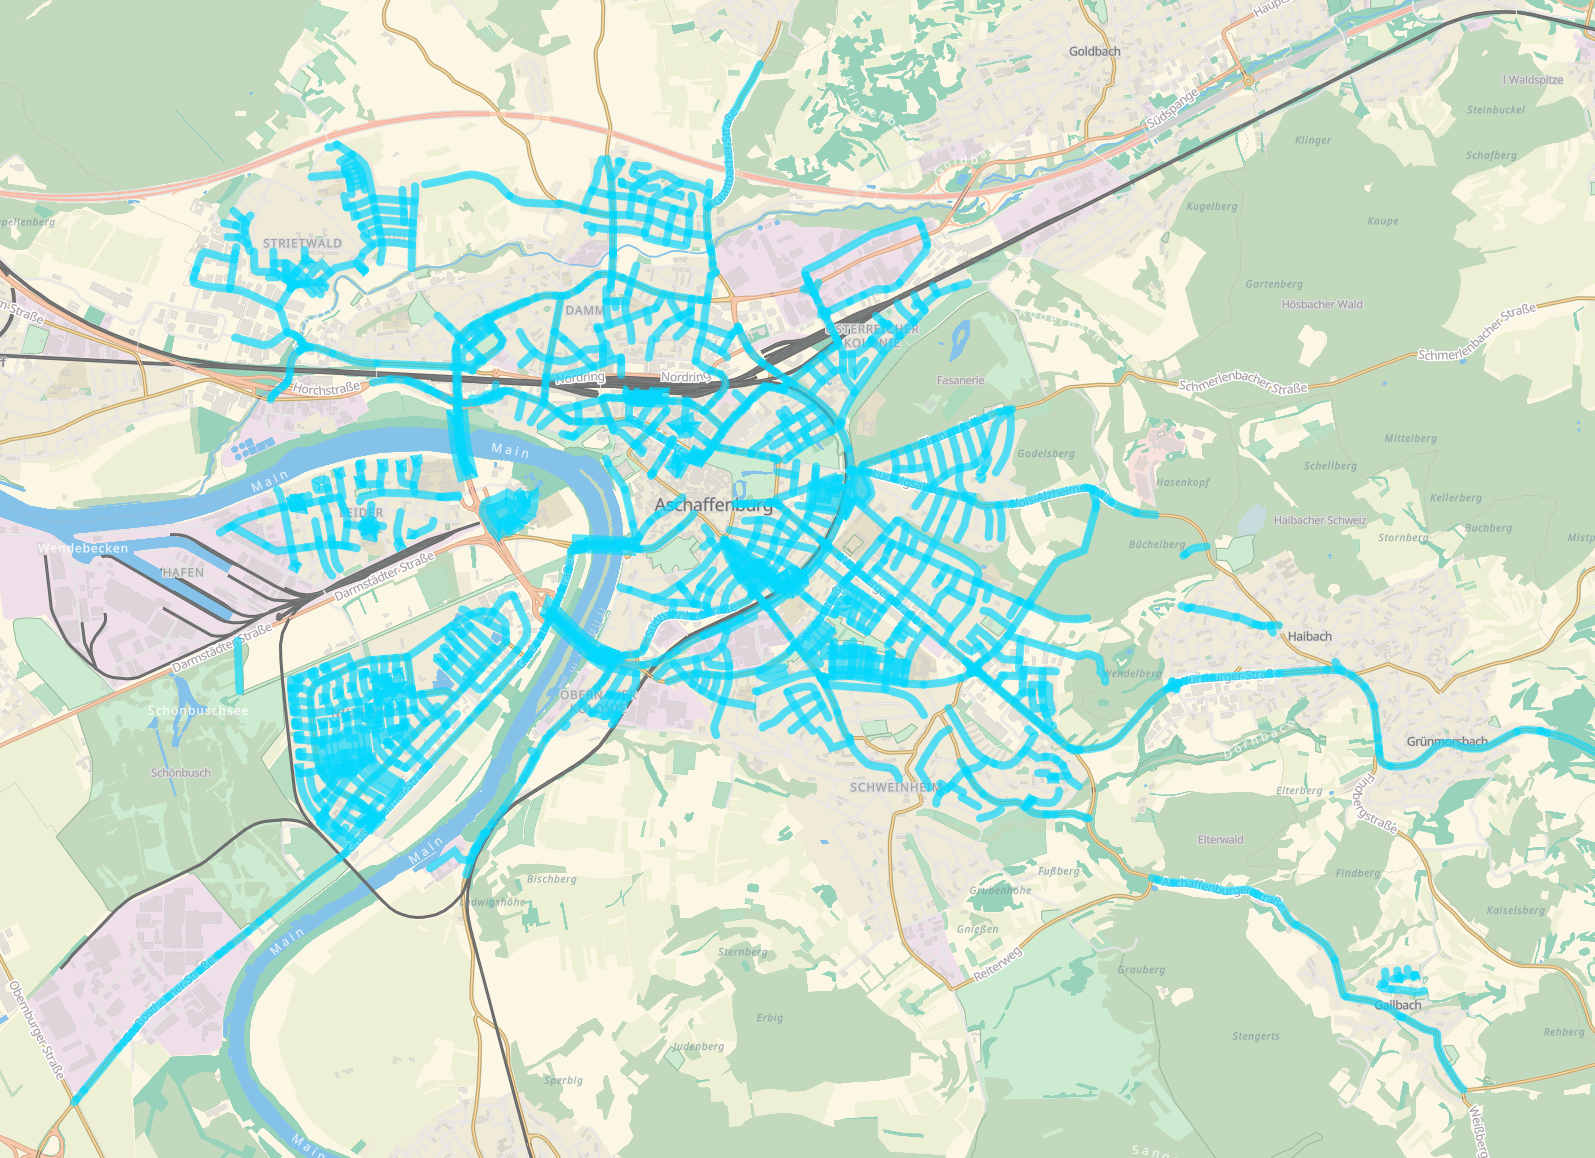
\includegraphics[width=1\linewidth]{0.png}
    \caption{Analysierte Straßen im Stadtgebiet mit jeweils blauer Hervorhebung.\footnote{\url{https://mapcomplete.org/etymology?z=13&lat=49.971624&lon=9.150400}}}
    \label{fig:map}
\end{figure}

\section{Vermeidung von Fehletymologien}
Um Fehlzuordnungen zu vermeiden, wie z.B. einer Straße zu einer Pflanze statt einer
Person, wird in der Regel darauf Rücksicht genommen, wonach die anderen Straßen in der
näheren Umgebung benannt sind. Dabei ist stets Achtsamkeit geboten, so sind
beispielsweise viele Straßen im Stadtteil Nilkheim nach Bäumen benannt, der
\texttt{Mergenbaum-Platz} inmitten dieser “Baumstraßen” aber nach einer Person. Durch
Überprüfung, ob ein Straßenname auf der Website des Stadtarchivs vermerkt ist sowie eine
zusätzliche Suche im Internet nach in Frage kommenden gleichnamigen Personen - auch
wenn ein nicht-menschliches Eponym offensichtlich erscheint - gehört also zur Sorgfalt bei
der Datenerhebung.

\section{Datenauswahl}
Für die Auswertung wird ein Programm in Python geschrieben. Dieses ruft zuerst die
Overpass-API (welche die OSM-Daten zur Verfügung stellt) mit folgender Query (Overpass
Query Language) ab:
\begin{lstlisting}
area["boundary"~"administrative"]
["de:place"~"city"]
["name"~"'+city+'"];
nwr["name:etymology:wikidata"](area);
out;
\end{lstlisting}

Diese Query gibt eine Liste aller Knoten (“nodes”), Strecken (“ways”) und Flächen (“areas”)
innerhalb des Verwaltungsbereichs der in der Variable "city" definierten Stadt (in diesem Fall "Aschaffenburg") zurück, die mit einem
“name:etymology:wikidata”-Tag versehen sind.
Da Straßen in OSM aus technischen Gründen oft keine durchgehenden Linien sind, sondern
oft unterbrochen werden (z.B. bei Änderungen der Anzahl der Spuren, bei
Fußgänger*innen-Überwegen, etc.), beinhaltet eine Straße oft mehrere Teilstrecken
(“ways”), die alle eine eindeutige Identifikationsnummer haben.
Die angefragten Daten von OSM werden iteriert und nach Straßennamen in einer Liste
sortiert, zusammen mit den zugehörigen Wikidata-IDs sowie den Way-IDs der Teilstrecken
von OSM.
Für jede Straße wird jeweils mit Hilfe der zugehörigen Way-IDs die Länge erhoben, was mit
folgendem Code erfolgt:
\begin{lstlisting}
def getLength(street):
  ids = db[street]["ids"]
  q = ",".join(str(x) for x in ids)
  fullq = "[out:json];way(id:"+q+");make stats length=sum(length());out;"
  url = "https://www.overpass-api.de/api/interpreter?data="+fullq
  r = requests.get(url)
  length = float(json.loads(r.content)["elements"][0]["tags"]["length"])
  return(length)
\end{lstlisting}

Nach Erhebung und Speicherung der Straßenlänge werden die Way-IDs aus dem Speicher
entfernt, da sie nicht weiter benötigt werden.
5
Im nächsten Schritt werden für jede auf diese Weise erhobene Straße die Wikidata-Einträge
der Eponyme, also der namensgebenden Entitäten, aufgerufen.
Die Datenstruktur von Wikidata besteht aus Properties und Entities, eine Entity besitzt
Properties, die wiederum in der Regel auf andere Entities verweisen, so beinhaltet z.B. die
Entität \texttt{Q481434 (Alfons Goppel)} die Property \texttt{P102 (Parteizugehörigkeit)}, welche wiederum
die Entitäten \texttt{Q49763 (CSU)}, \texttt{Q7320 (NSDAP)} und \texttt{Q302884 (BVP)} beinhaltet. Ebenso
enthält \texttt{Q481434 (Alfons Goppel)} auch eine Property \texttt{P21 (Geschlecht)}, welche in diesem
Fall \texttt{Q6581097 (männlich)} beinhaltet, sowie eine Property \texttt{P31 (ist ein/e)}, die hier \texttt{Q5
(Mensch)} beinhaltet. \texttt{P31} ist deshalb von Bedeutung, weil sie auch z.B. eine Stadt oder
Gemeinde, ein Gebirge, ein Fluss, eine Tiergattung, etc. sein kann. Die API-Abfrage erfolgt
mit Hilfe der Python-Bibliothek “Wikibase Integrator”\footnote{\url{https://github.com/LeMyst/WikibaseIntegrator}}.
Auf diese Weise werden also für alle Straßen für alle jeweiligen Eponyme der Typ (\texttt{ist
ein/e}) erhoben - sowie für Menschen jeweils dazugehörige Geschlechter, ausgeübte
Tätigkeiten sowie die Parteizugehörigkeiten - und zu den einzelnen Straßen in eine Datei
abgespeichert.
Eine so verarbeitete Straße sieht im analysierbaren Endzustand im JSON-Format also z.B.
so aus:
\begin{lstlisting}
"Albrecht-Velte-Straße": {
  "wikidata": [
    {
      "type": "Q5",
      "id": "Q125996420",
      "name": "Albrecht Velte",
      "genders": [
        "Q6581097"
      ],
      "parties": [
        "Q7320",
        "Q49763"
      ],
      "jobs": [
        "Q51073447",
        "Q4991371",
        "Q110242307",
        "Q30185"
      ],
      "birthday": {
        "year": 1920,
        "month": 6,
        "day": 17
      },
      "deathday": {
        "year": 1992,
        "month": 9,
        "day": 14
      },
      "age": 72
    }
  ],
  "length": 116.507
}
\end{lstlisting}

Die Größe dieser zu diesem Zweck erstellten Datei beträgt gut 150 kB und beinhaltet 8175
Zeilen. Eine separate lokale Datenbank mit den jeweiligen Namen der Wikidata-IDs wurde aus zwei Gründen angelegt:
Zum Einen erspart dies redundaten Netzwerkverkehr zur Wikidata-API, zum Anderen lassen sich so die Namen per Hand
lokal modifizieren. Dies ist relevant, da Wikidata standardmäßig keine diskriminierungsfreien Berufsbezeichnungen bereitstellt.

\section{Datenauswertung}
In einem zweiten Schritt wird die zuvor erstellte Datei als Grundlage für die Erstellung
der abschließenden Statistiken verwendet. Auch dieses Programm ist in Python
geschrieben.
Es werden dabei unter Anderem folgende Zahlen erhoben:

\subsection{Gesamtzahl der Straßen mit “name:etymology:wikidata”-Tags im
Verwaltungsgebiet Aschaffenburg}
Berechnung:
\begin{lstlisting}
for street in db:
  totalStreets = totalStreets+1
\end{lstlisting}
Die resultierende natürliche Zahl gibt an, wie viele Straßen insgesamt erfasst wurden.

\subsection{Addierte Gesamtlänge der Straßen mit “name:etymology:wikidata”-Tags
im Verwaltungsgebiet Aschaffenburg}
Berechnung:
\begin{lstlisting}
for street in db:
  totalStreetLength = totalStreetLength + db[street]["length"]
\end{lstlisting}
Die resultierende Fließkommazahl gibt die Gesamtlänge aller erfassten Straßen in Metern
an.

\subsection{Gesamtzahl der menschlichen Eponyme von Straßen im
Verwaltungsgebiet Aschaffenburg}
Berechnung:
\begin{lstlisting}
for street in db:
  for entity in db[street]["wikidata"]:
    if entity["type"] == "Q5":
      totalHuman = totalHuman+1
\end{lstlisting}
Die resultierende Zahl gibt an, wie viele Menschen insgesamt namensgebend für Straßen
sind.

\subsection{Die jeweilige Gesamtzahl der von menschlichen Eponymen von Straßen
im Verwaltungsgebiet Aschaffenburg verwendeten Geschlechter}
Berechnung:
\begin{lstlisting}
genderCounts = {}
for street in db:
  for entity in db[street]["wikidata"]:
    if "genders" in entity:
      for gender in entity["genders"]:
        if gender in genderCounts:
          genderCounts[gender] = genderCounts[gender] + 1
        else:
          genderCounts[gender] = 1
\end{lstlisting}
Das resultierende Dictionary enthält als Schlüssel die Entitäts-IDs von Geschlechtern, sowie
als Werte die addierte Anzahl (als natürliche Zahl), wie oft Eponyme das jeweilige
Geschlecht haben.

\subsection{Die jeweilige Gesamtzahl der von menschlichen Eponymen von Straßen
im Verwaltungsgebiet Aschaffenburg vertretenen politischen Parteien}
Berechnung:
\begin{lstlisting}
partyCounts = {}
for street in db:
  for entity in db[street]["wikidata"]:
    if "parties" in entity:
      for party in entity["parties"]:
        if party in partyCounts:
          partyCounts[party] = partyCounts[party]+1
        else:
          partyCounts[party] = 1
\end{lstlisting}
Das resultierende Dictionary enthält als Schlüssel die Entitäts-IDs von politischen Parteien,
sowie als Werte die addierte Anzahl (als natürliche Zahl), wie oft Eponyme der jeweiligen
Partei zugehörig sind.

\subsection{Die jeweilige Gesamtlänge von Straßen mit
“name:etymology:wikidata”-Tags im Verwaltungsgebiet Aschaffenburg,
getrennt nach Geschlecht der jeweiligen Eponyme}
Berechnung:
\begin{lstlisting}
streetLengthsByGender = {}
humanStreetLength = 0
for street in db:
  for entity in db[street]["wikidata"]:
    if entity["type"] == "Q5":
      humanStreetLength = humanStreetLength + db[street]["length"]
    if "genders" in entity:
      for gender in entity["genders"]:
        if gender in streetLengthsByGender:
          streetLengthsByGender[gender] =
streetLengthsByGender[gender]+db[street]["length"]
        else:
          streetLengthsByGender[gender] = db[street]["length"]
\end{lstlisting}
Das resultierende Dictionary enthält als Schlüssel die Entitäts-IDs von Geschlechtern, sowie
als Werte die addierte Länge (als Fließkommazahl) aller Straßen in Metern, deren Eponyme
das jeweilige Geschlecht haben.

\subsection{Gesamtzahl der menschlichen Eponyme von Straßen im
Verwaltungsgebiet Aschaffenburg, die weder ein cis-männliches noch
cis-weibliches Geschlecht haben}
Berechnung:
\begin{lstlisting}
diverseGendersAmount = 0
for street in db:
  for entity in db[street]["wikidata"]:
    if "genders" in entity:
      for gender in entity["genders"]:
        if not gender == "Q6581097" and not gender == "Q6581072":
          diverseGendersAmount = diverseGendersAmount + 1
\end{lstlisting}
Die resultierende natürliche Zahl gibt an, wie viele Eponyme weder ein cis-männliches noch
ein cis-weibliches Geschlecht haben.

\subsection{Die jeweilige Gesamtzahl der von menschlichen Eponymen von Straßen
im Verwaltungsgebiet Aschaffenburg ausgeübten Tätigkeiten}
Berechnung:
\begin{lstlisting}
jobsCounts = {}
for street in db:
  for entity in db[street]["wikidata"]:
    if "jobs" in entity:
      for job in entity["jobs"]:
        if job in jobsCounts:
          jobsCounts[job] = jobsCounts[job]+1
        else:
          jobsCounts[job] = 1
\end{lstlisting}
Das resultierende Dictionary enthält als Schlüssel die Entitäts-IDs von Tätigkeiten, sowie als
Werte die addierte Anzahl (als natürliche Zahl), wie oft Eponyme die jeweilige Tätigkeit
ausüben.

Der gesamte Quellcode des Scripts ist öffentlich\footnote{\url{https://github.com/MeltedHugo/gender-gapped-street-names/}}, die Analyse kann reproduziert werden.


\section{Ergebnisse}

\begin{figure}
  \centering
  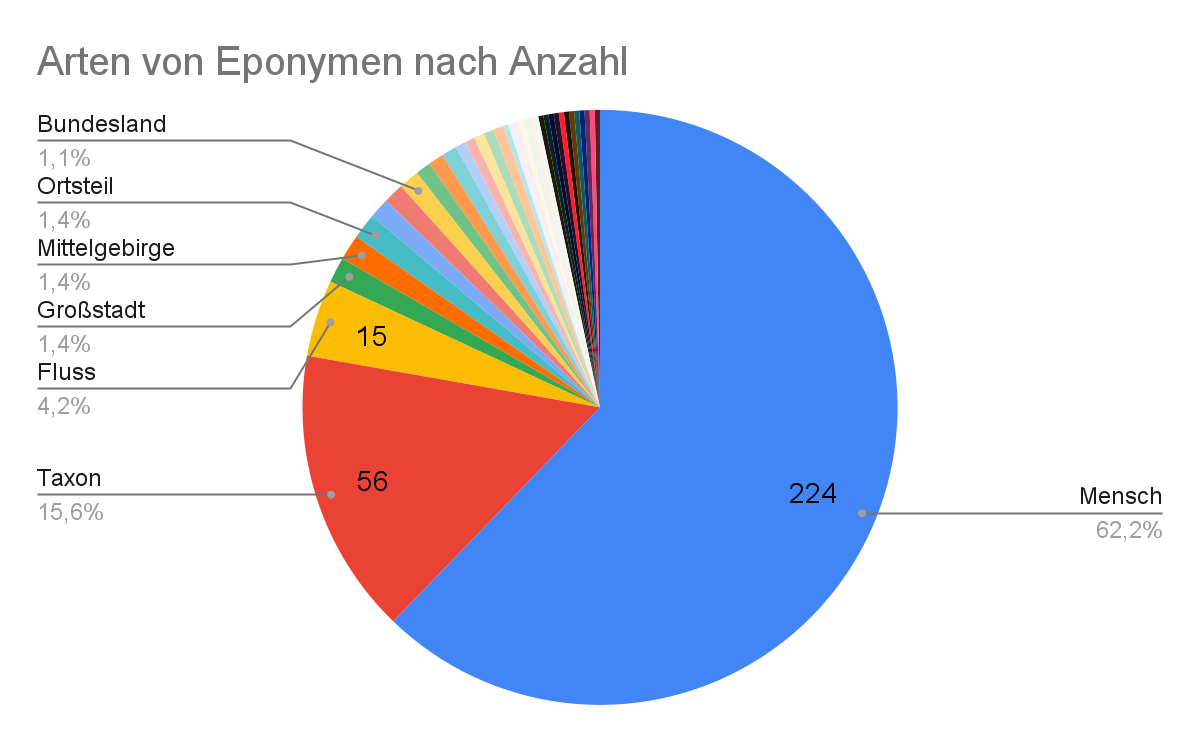
\includegraphics[width=1\linewidth,frame]{1.png}
  \caption{Arten von Eponymen nach Anzahl}
  \label{fig:TypesByCount}
\end{figure}
\begin{figure}
  \centering
  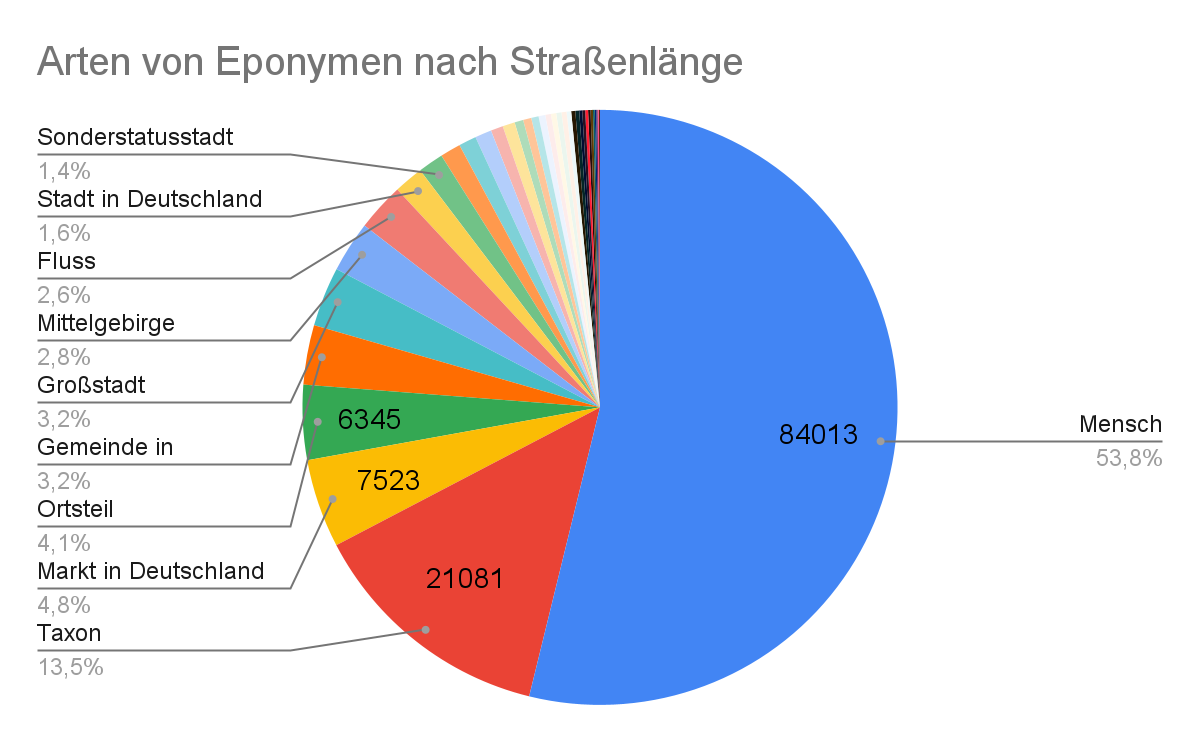
\includegraphics[width=1\linewidth,frame]{2.png}
  \caption{Arten von Eponymen nach Straßenlänge}
  \label{fig:TypesByLength}
\end{figure}

\begin{figure}
\centering
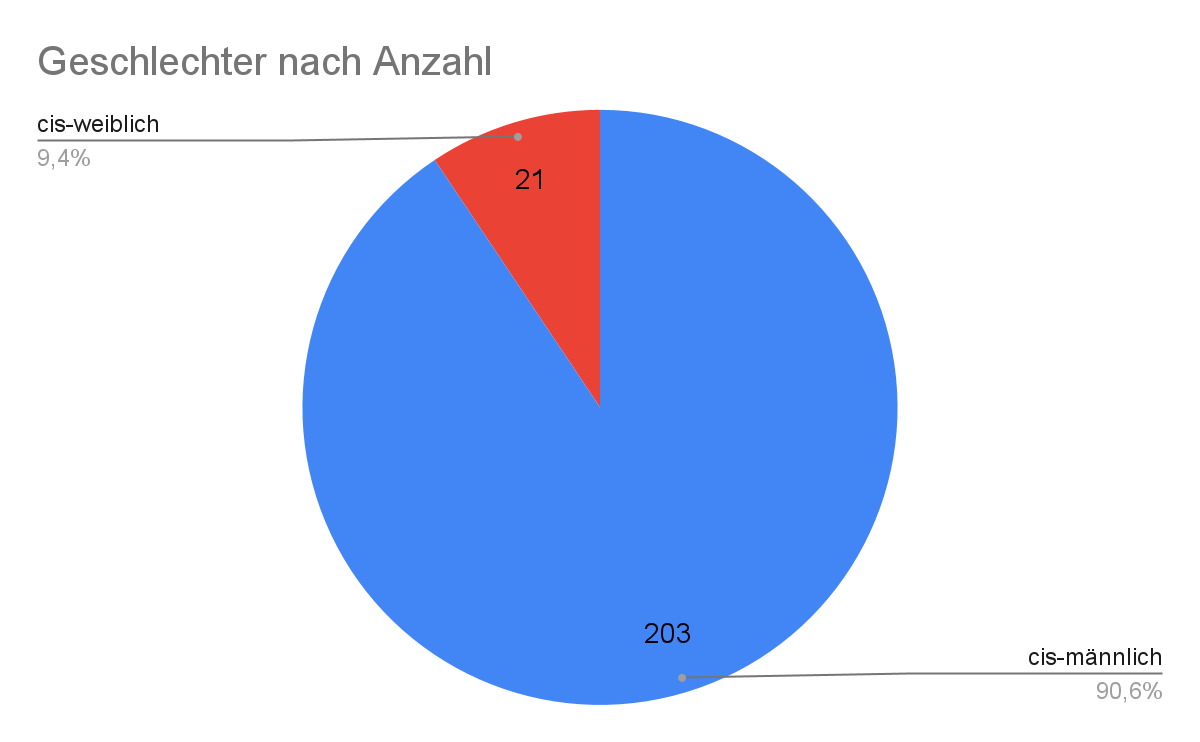
\includegraphics[width=1\linewidth,frame]{3.png}
\caption{Geschlechter nach Anzahl}
\label{fig:GendersByCount}
\end{figure}
\begin{figure}
\centering
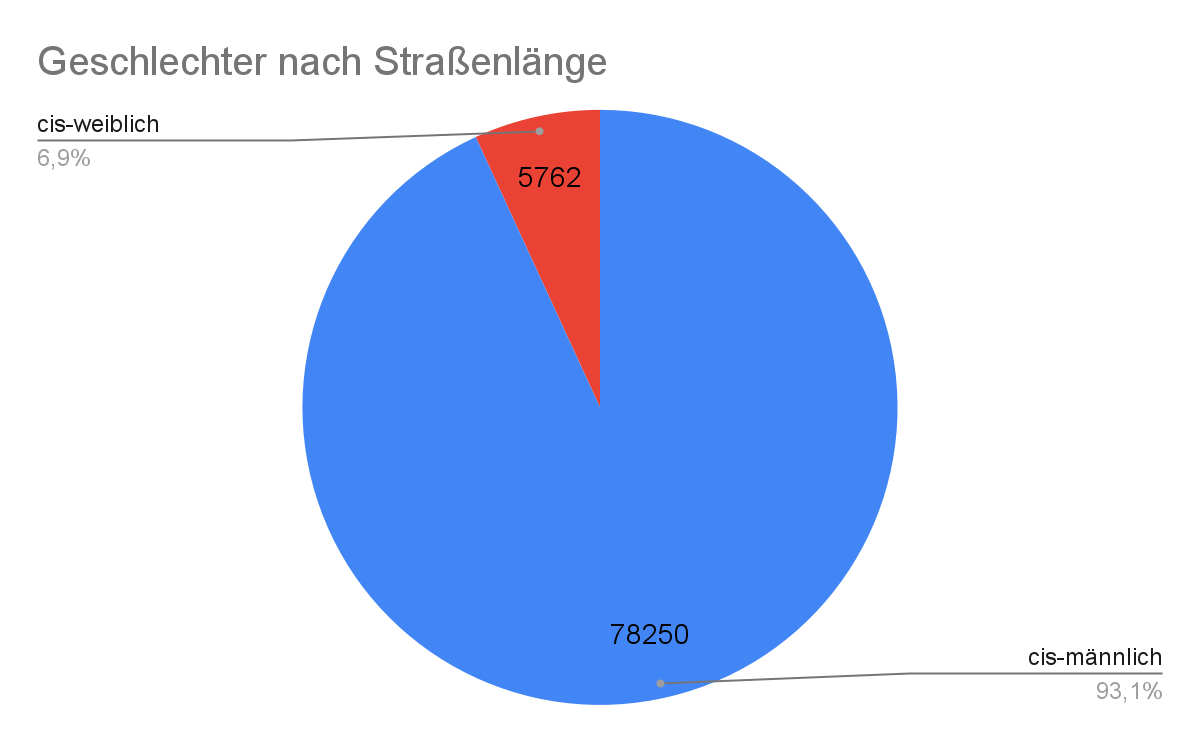
\includegraphics[width=1\linewidth,frame]{4.png}
\caption{Geschlechter nach Straßenlänge}
\label{fig:GendersByLength}
\end{figure}

\begin{figure}
\centering
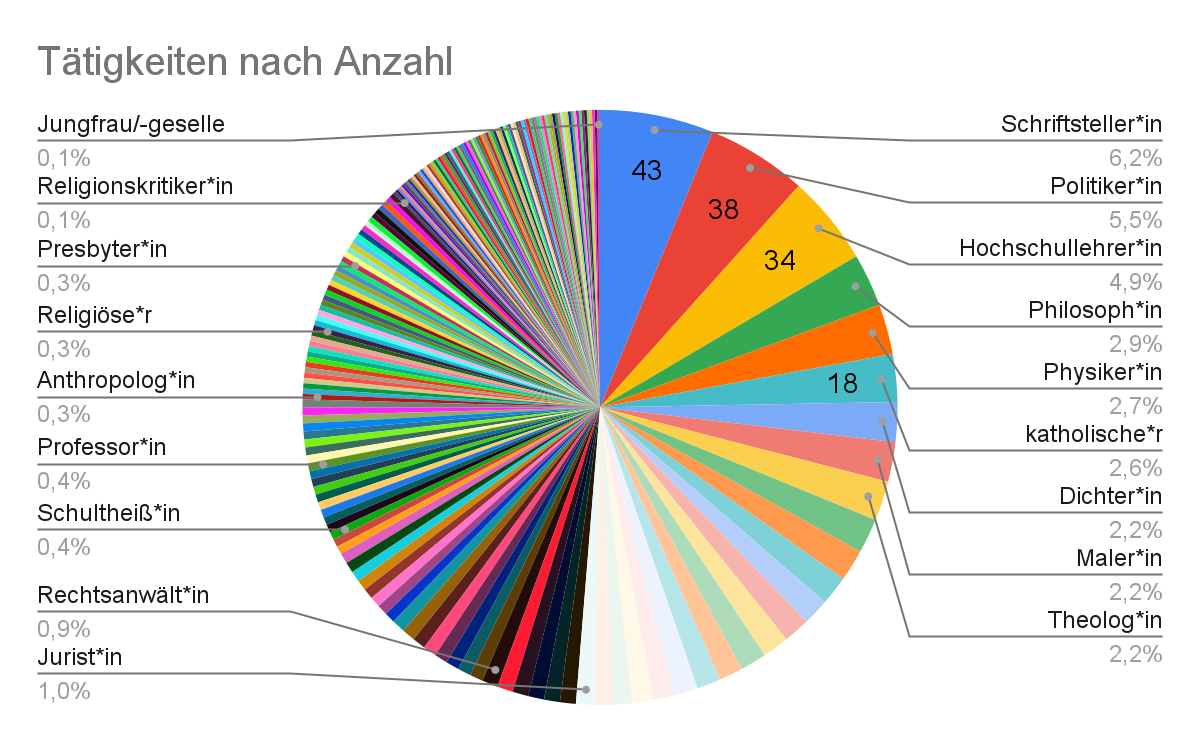
\includegraphics[width=1\linewidth,frame]{5.png}
\caption{Tätigkeiten nach Anzahl}
\label{fig:JobsByCount}
\end{figure}
\begin{figure}
\centering
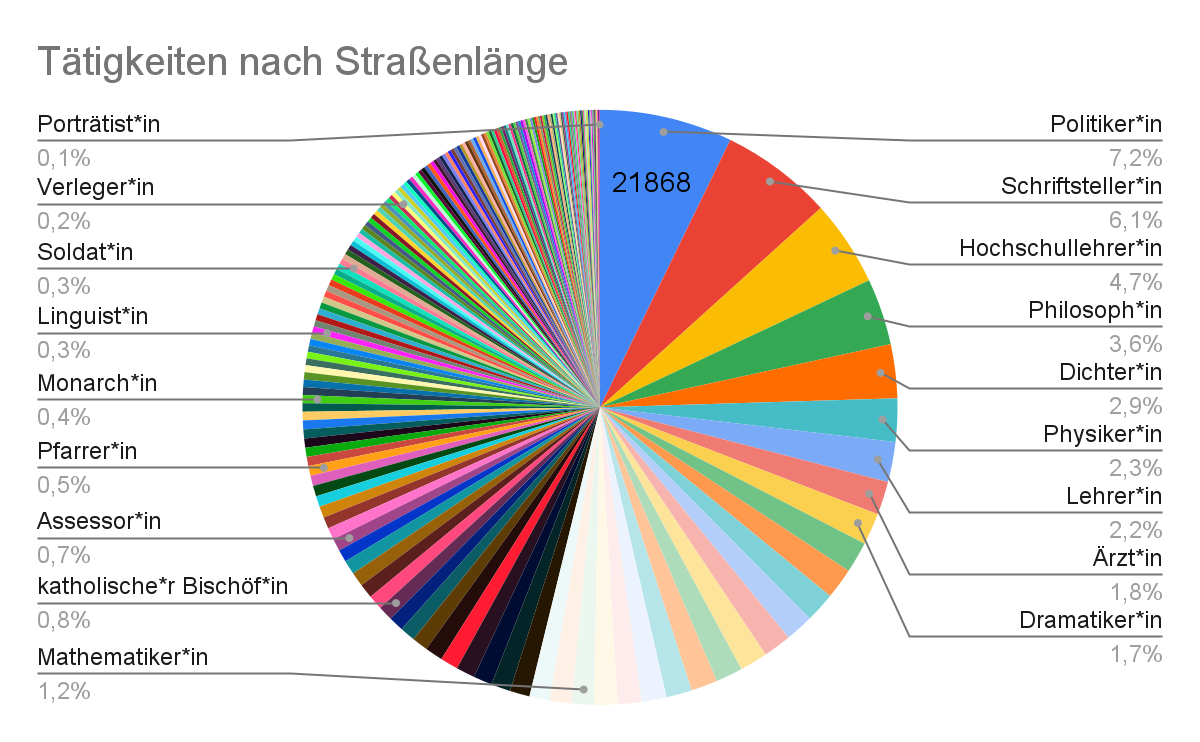
\includegraphics[width=1\linewidth,frame]{6.png}
\caption{Tätigkeiten nach Straßenlänge}
\label{fig:JobsByLength}
\end{figure}

\begin{figure}
\centering
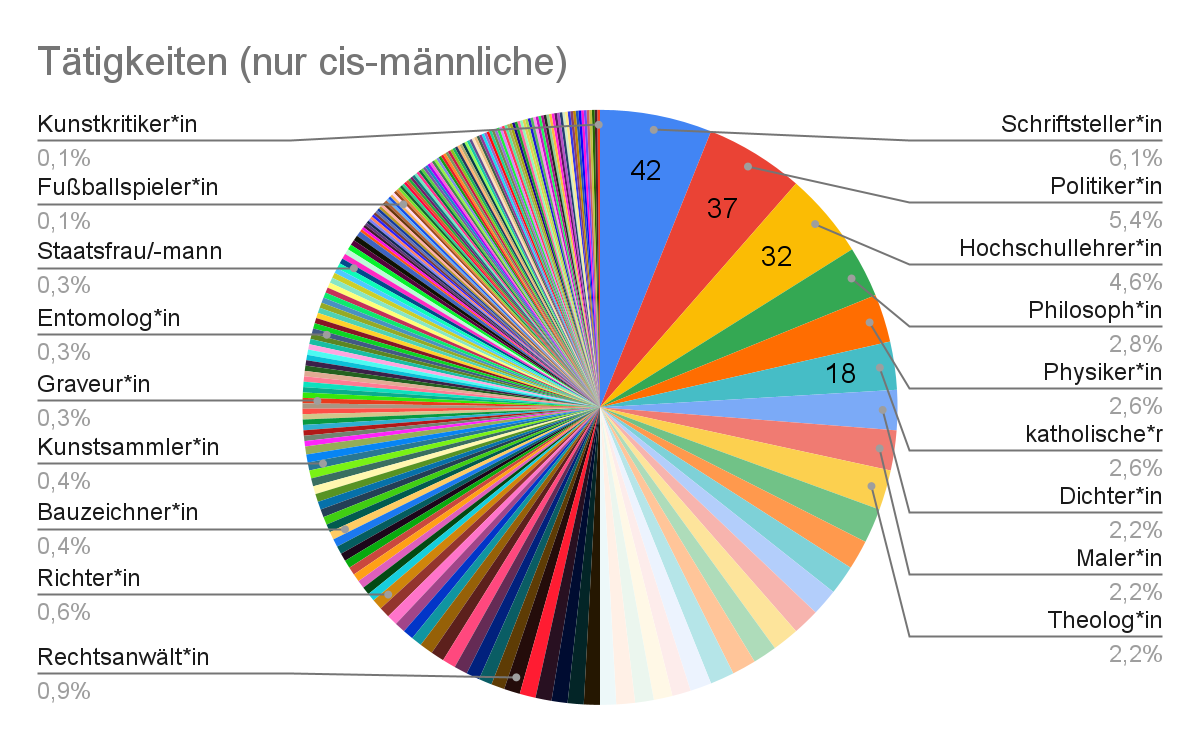
\includegraphics[width=1\linewidth,frame]{7.png}
\caption{Tätigkeiten (nur cis-männliche)}
\label{fig:JobsOnlyMale}
\end{figure}
\begin{figure}
\centering
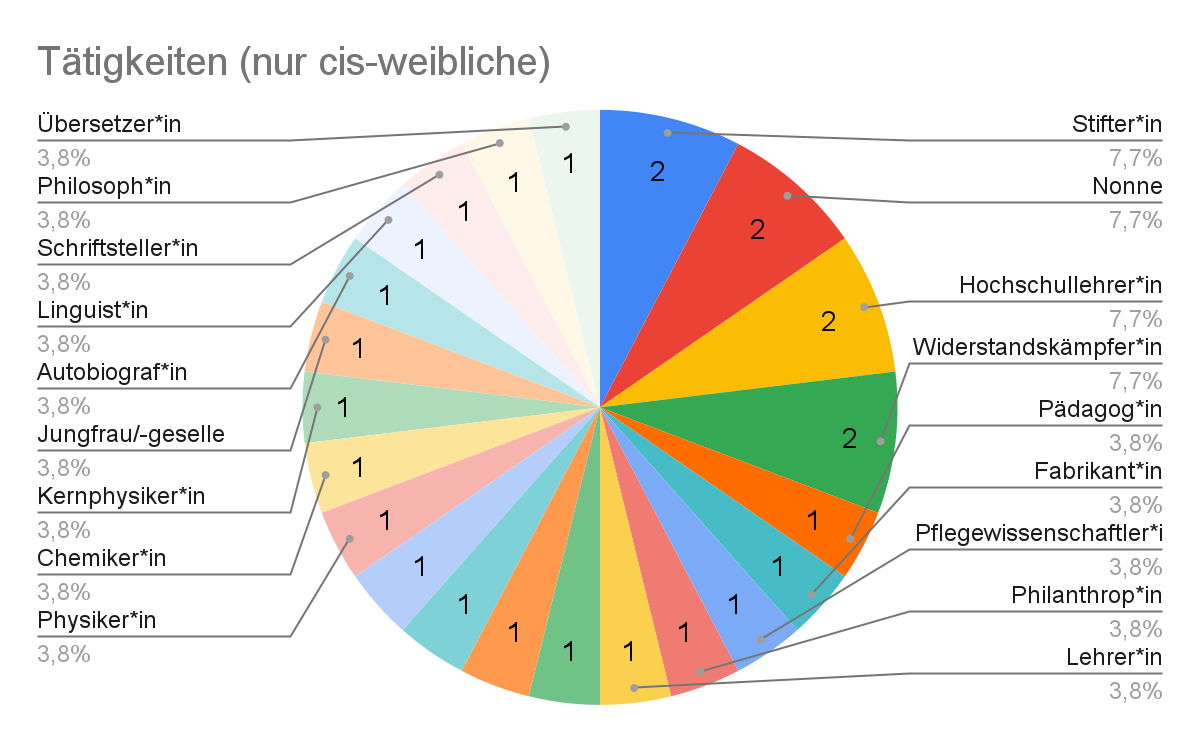
\includegraphics[width=1\linewidth,frame]{8.png}
\caption{Tätigkeiten n(nur cis-weibliche)}
\label{fig:JobsOnlyFemale}
\end{figure}

\begin{figure}
\centering
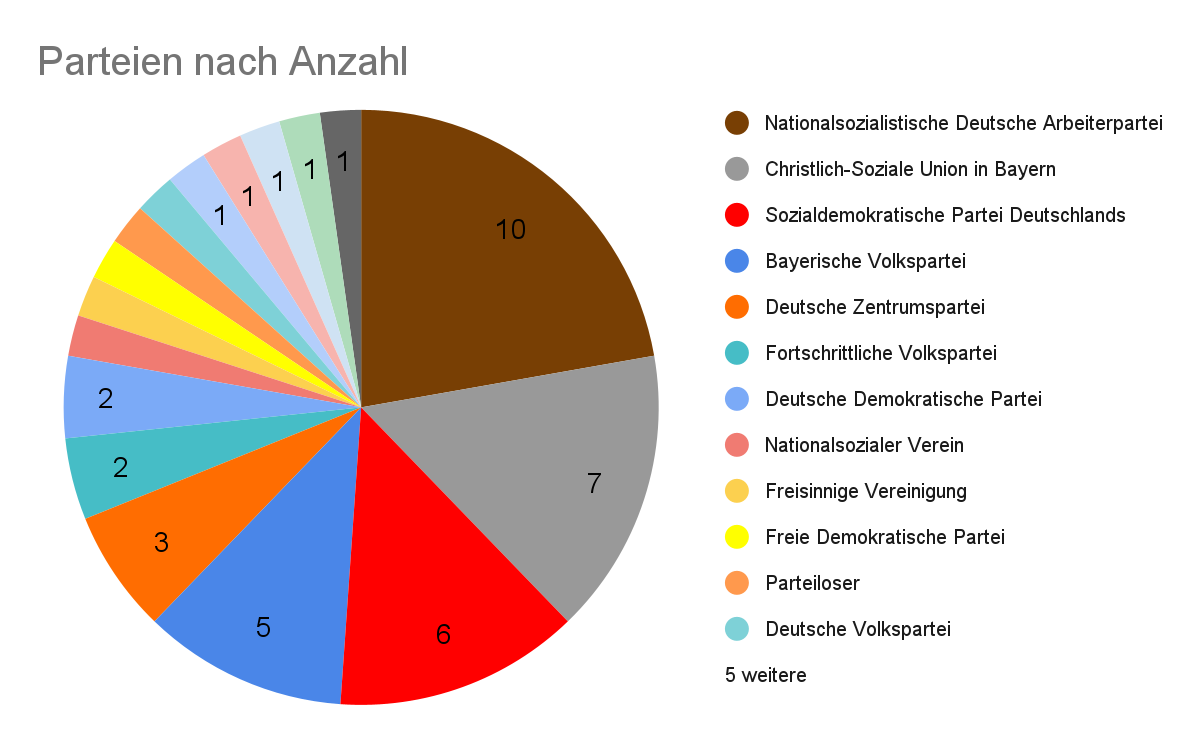
\includegraphics[width=1\linewidth,frame]{9.png}
\caption{Parteien nach Anzahl}
\label{fig:PartiesByCount}
\end{figure}
\begin{figure}
\centering
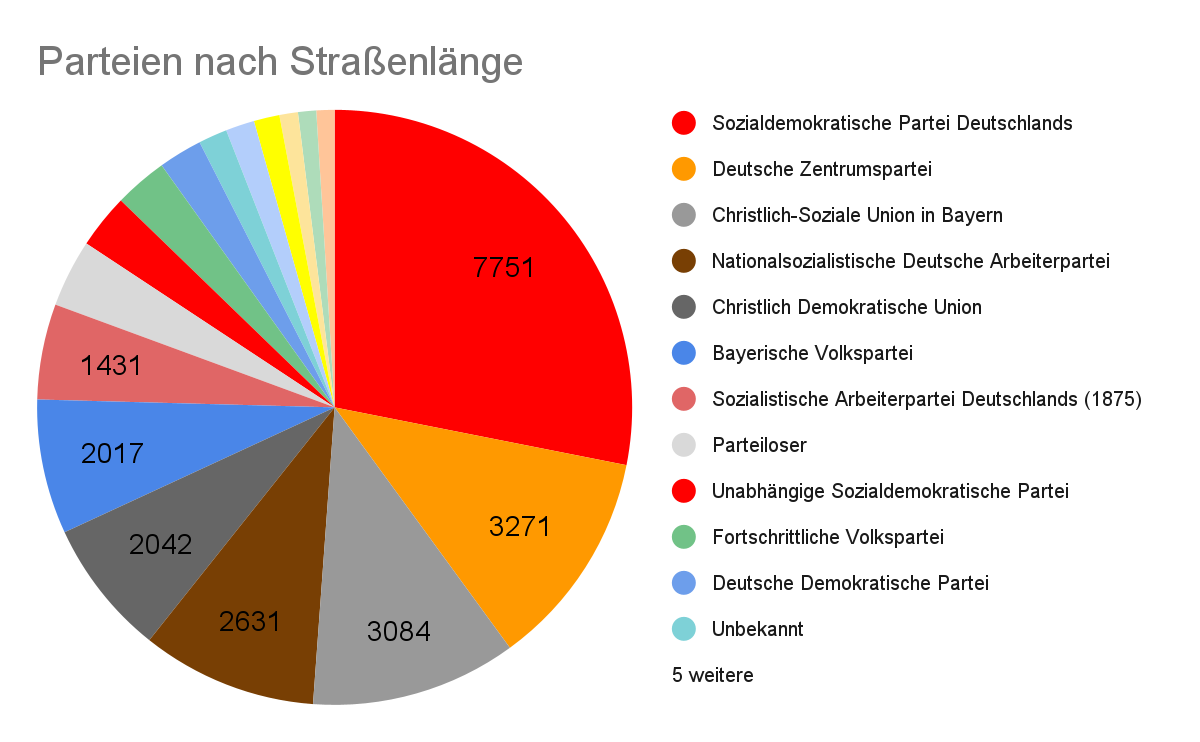
\includegraphics[width=1\linewidth,frame]{10.png}
\caption{Parteien nach Straßenlänge}
\label{fig:PartiesByLength}
\end{figure}

Insgesamt wurden im Stadtbereich Aschaffenburg (Innenstadt, Strietwald, Damm,
Österreicher Kolonie, Leider, Hafen, Nilkheim inkl. Industriegebiet Nilkheim, Obernauer
Kolonie, Schweinheim und Gailbach) 357 Straßen, Plätze, Schulen und ähnliche Orte
(“Straßen”) erfasst (siehe Abbildung~\ref{fig:map}).\\
62,2 \% der erfassten Straßen sind nach Menschen benannt, 15,6 \% nach Tier- oder
Pflanzengattungen (siehe Abbildung~\ref{fig:TypesByCount}). Diese Verteilung gestaltet sich ähnlich, wenn statt der Anzahl die
addierte Länge der jeweiligen Straßen betrachtet wird, hier sind ca. 84 km nach Menschen
und 21 km nach Tier- oder Pflanzengattungen benannt (siehe Abbildung~\ref{fig:TypesByLength}).



Von den Straßen, die nach Menschen benannt sind, wurden 90,6 \% nach cis-männlichen
und 9,4 \% nach cis-weiblichen Menschen benannt (siehe Abbildung~\ref{fig:GendersByCount}). Wird statt der Anzahl die Straßenlänge
betrachtet, ist der Unterschied etwas größer (93,1 \% cis-männlich bzw. 6,9 \% cis-weiblich) (siehe Abbildung~\ref{fig:GendersByLength}).
Es gibt keinen einzigen Fall, in dem andere Geschlechter bei der Namensgebung
berücksichtigt wurden.
Die Dominanz cis-männlicher Geschlechter stellt eine Diskrepanz zur amtlichen
Bevölkerungsstatistik dar (49,2 \% männlich / 50,7 \% weiblich)\footnote{\url{https://www.destatis.de/DE/Themen/Gesellschaft-Umwelt/Bevoelkerung/Bevoelkerungsstand/Tabellen
/deutsche-nichtdeutsche-bevoelkerung-nach-geschlecht-deutschland.html}} dar. Da das
Selbstbestimmungsgesetz noch nicht in Kraft getreten ist und es daher eine Dunkelziffer
gibt, können diversgeschlechtliche Menschen noch nicht repräsentativ in der
Vergleichsstatistik berücksichtigt werden.



Die am häufigsten von Namensgeber*innen ausgeübten Tätigkeiten sind: Schriftsteller*in
(6,2 \%), Politiker*in (5,5 \%) und Hochschullehrer*in (4,9 \%) (siehe Abbildung~\ref{fig:JobsByCount}). Wird statt der Anzahl die
Straßenlänge betrachtet, so sind Politiker*innen mit 7,2 \% bzw. 21,8 km am stärksten
vertreten - der Willi-Reiland-Ring spielt hier vermutlich eine bedeutende Rolle (siehe Abbildung~\ref{fig:JobyByLength}).



Die Tätigkeiten der Namensgeber*innen wurden anschließend noch nach Geschlechtern
unterteilt. Während es keine Auffälligkeiten unter cis-männlichen Namensgebern gibt (Abbildung~\ref{fig:JobsOnlyMale}), so
sieht die Datenlage unter cis-weiblichen Namensgeberinnen dürftig aus (Abbildung~\ref{fig:JobsOnlyFemale}). Am häufigsten sind
Stifterinnen, Nonnen, Hochschullehrerinnen und Widerstandskämpferinnen mit jeweils
lediglich zwei Straßen vertreten.



Die Parteizugehörigkeit von Namensgeber*innen, die nachweislich Mitglied einer Partei
waren, wurde ebenfalls untersucht (Abbildung~\ref{fig:PartiesByCount}). Die Partei, die dabei im Stadtgebiet Aschaffenburg mit
20,41 \% am häufigsten vertreten ist, ist die NSDAP, mit zehn Namensgebern (Matthäus
Hotzel, Julius Maria Becker, Paul Rudolf Scheppler, Hans Hönlein, Christian Schad, Ludwig
Roth, Ernst Streun, Albrecht Velte, Aloys Lautenschläger, Alfons Goppel). Es fanden sich
darunter auch Namensgeber, die Mitglied der SS und/oder der SA waren, es fanden sich
aber auch Wehrmachtssoldaten, zu denen keine NSDAP-Mitgliedschaft überliefert ist.
Wird statt der Anzahl die Länge betrachtet, so ändert sich die Verteilung, auch hier spielt der
Willi-Reiland-Ring sowie die Mainbrücken vermutlich eine bedeutende Rolle (Abbildung~\ref{fig:PartiesByLength}). Nach
NSDAP-Mitgliedern sind insgesamt etwa 2,6 km benannt.


\section{Einschränkungen und Ausblick}
Aufgrund von Zeitmangel konnten die Straßen im Stadtteil Obernau nicht rechtzeitig
analysiert werden. Was bei der Kategorisierung der Ergebnisse nicht berücksichtigt werden
konnte, war die ungefähre Anzahl der Einwohner*innen in einer Straße. Die Schätzung
dieser Daten erfordert weitergehende Arbeit, die die Erhebung der jeweiligen Gebäude im
Hinblick auf ihren Typ (Ein-/Mehrfamilienhaus, Doppelhaushälfte, etc) und Anzahl der
jeweiligen Stockwerke erfordert, sowie eine Auskunft über die durchschnittliche
Einwohnerzahl pro Quadratmeter Wohnfläche im jeweiligen Gebäudetyp. Eine derartige
Erhebung nach diesen Kriterien würde zu weiteren interessanten Ergebnissen führen, da so
z.B. der Ring, die Brücken und ähnlich “unbewohnte” Straßen vernachlässigt werden und
stark “bewohnte” Straßen ungeachtet ihrer Länge wesentlich schwerer ins Gewicht fallen.
Eine weitergehende Untersuchung in diese Richtung ist beabsichtigt, konnte aber aufgrund
des hohen Aufwands nicht rechtzeitig abgeschlossen werden.
Ein weiterer Aspekt, dessen Untersuchung interessant ist, ist die Aufschlüsselung nach
Stadtteilen bzw. Vierteln. Dies ist mit der aktuellen Datenlage möglich und wird ebenfalls Teil
zukünftiger Forschung sein.

\section{Appell}
Da die Stadt Aschaffenburg bereits auf das Thema aufmerksam geworden ist und sich bald
mit einigen Umbenennungen beschäftigen wird, möchte ich mit Hilfe dieser Untersuchung
dazu aufrufen, die anstehenden Straßennamensänderungen vor allem Frauen (und gerne
auch diversgeschlechtlichen Menschen) zu widmen und dabei nicht nur deren eventuelles
Wirken im (bzw. gegen den) Nationalsozialismus zu untersuchen, sondern deren generelle
Einstellung gegenüber fundamentalen Fragen wie Menschenrechten oder deren Bedeutung
für die Stadt Aschaffenburg.
Straßennamen haben einen repräsentativen Charakter. Wenn die Stadt Aschaffenburg eine
weltoffene, moderne Stadt sein möchte, sollte sie das auch zeigen. Der Weg zu vollständiger
und tatsächlicher Gleichberechtigung ist lang und schwer, aber es gibt genügend
Möglichkeiten, wo damit angefangen werden kann.


\appendix
\section{Rohdaten}
\subsection{Eponyme nach Anzahl}
\csvautobooklongtable{../csv/TypesByNumbers.csv}
\subsection{Eponyme nach Straßenlänge}
\csvautobooklongtable{../csv/TypesByLength.csv}
\subsection{Geschlechter nach Anzahl}
\csvautobooklongtable{../csv/GendersByNumbers.csv}
\subsection{Geschlechter nach Straßenlänge}
\csvautobooklongtable{../csv/GendersByLength.csv}
\subsection{Tätigkeiten nach Anzahl}
\csvautobooklongtable{../csv/JobsByNumbers.csv}
\subsection{Tätigkeiten nach Straßenlänge}
\csvautobooklongtable{../csv/JobsByLength.csv}
\subsection{Tätigkeiten (nur cis-männliche)}
\csvautobooklongtable{../csv/JobsOnlyMale.csv}
\subsection{Tätigkeiten (nur cis-weibliche)}
\csvautobooklongtable{../csv/JobsOnlyFemale.csv}
\subsection{Parteien nach Anzahl}
\csvautobooklongtable{../csv/PartiesByNumbers.csv}
\subsection{Parteien nach Straßenlänge}
\csvautobooklongtable{../csv/PartiesByLength.csv}
%\subsection{Personen, die einer Tätigkeit bzw. Partei zugehörig sind}
%\VerbatimInput{../people.json}
%\subsection{Menschenlesbare Datenbank}
%\VerbatimInput{../readable_db.json}


\end{document}